\chapter{Multiscale turbulence measurements}
\label{ch:TurbulenceMeasurements}
Development of a first-principles understanding
of turbulent transport in a tokamak
requires multi-tiered validation\ldots
comparing not just heat fluxes, but
also turbulent spectra etc.
\diiid's extensive suite of fluctuation diagnostics
provides an ideal setting to validate
predicted changes~\cite{howard_pp16}
to turbulent spectra when altering relative drive
between electron-scale and ion-scale turbulence.


\section{Overview of multiscale gyrokinetic predictions}


\section{Experimental conditions}
The experiment was run in the ITER-similar shape,
with aspect ratio, elongation, and triangularity
all closely matched to those of the ITER-baseline scenario
\cite[Sec.~13.5 \& 13.6]{wesson}.
The on-axis toroidal field $B_T = \SI{1.7}{\tesla}$ and
plasma current $I_p = \SI{1.3}{\mega\ampere}$
produced $q_{95} = 3.15$,
where $q_{95}$ is the average value
of the safety factor $q$~\cite[Sec.~3.4]{wesson}
over the surface that encloses $95\%$
of the poloidal flux within the last-closed flux surface.
Neutral beam injection (NBI)~\cite[Sec.~5.3-5.5]{wesson}
was performed with feedback to maintain
$\beta_N = 1.9$, where
$\beta_N$ is the normalized plasma pressure~\cite[Sec.~6.18]{wesson}.
In order to suppress core MHD,
an average NBI torque of approximately $\SI{1.5}{\newton \meter}$
was injected into the plasma;
note that this is approximately four times larger than
the projected ITER-equivalent torque~\cite{garofalo_nf11}.
In order to alter the local electron-scale and ion-scale drives,
the electron cyclotron resonance heating (ECH)~\cite[Sec.~5.10]{wesson}
location was scanned between $\rho = 0.5$ and $\rho = 0.8$,
where $\rho$ is the square root of the normalized toroidal flux
(which scales as $r / a$, with
$r$ being the minor-radial coordinate and
$a$ being the minor radius of the plasma).
Intra-shot scans of the ECH location
were plagued with core MHD, so
only shot-to-shot, MHD-free scans of the ECH location
are considered here.
The line-averaged density was
$\bar{n}_e = \SI{5.2e19}{\per\meter\cubed}$.
Impurities were removed from the plasma
by both large and small edge localized modes (ELMs)~\cite[Sec.~7.17]{wesson}.
The time histories of several actuators and plasma parameters
are shown in Figure~\ref{fig:TurbulenceMeasurements:traces}.
Note that multiscale gyrokinetic simulations
of this experiment's reference discharge,
\diiid\space shot $153523$ with ECH at $\rho = 0.5$,
indicate that the turbulent transport
is intrinsically multiscale in nature~\cite{holland_nf17}.

\begin{figure}
  \centering
  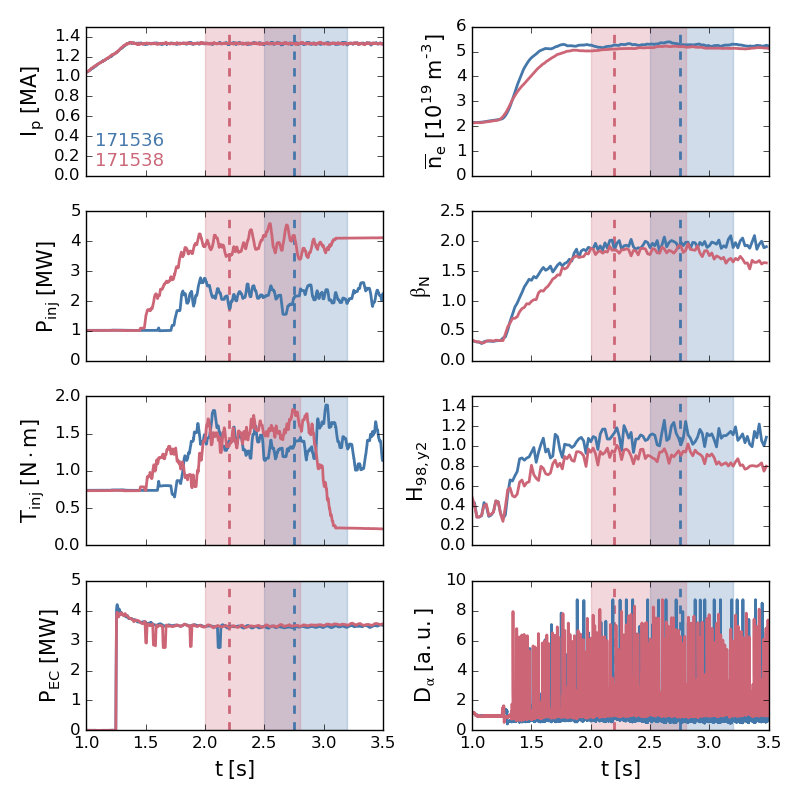
\includegraphics[width = \textwidth]{%
    Chapters/TurbulenceMeasurements/figs/traces.png}
  \caption[Time histories of various actuators \& plasma parameters]{%
    Time histories of various actuators and plasma parameters:
    (a) electron cyclotron resonance heating (ECH) power $P_{\text{ECH}}$,
    (b) ECH location $\rho_{\text{ECH}}$,
    (c) neutral beam injected (NBI) power $P_{\text{inj}}$,
    (d) NBI torque $T_{\text{inj}}$,
    (e) line-averaged density $\bar{n}_e$,
    (f) normalized plasma pressure $\beta_N$,
    (g) confinement quality $H_{98,\text{y}2}$, and
    (h) divertor $D_{\alpha}$ light, indicating
    the presence of large and small edge localized modes (ELMs).
  }
\label{fig:TurbulenceMeasurements:traces}
\end{figure}

Equilibrium profiles were obtained
by averaging over $\SI{200}{\milli\second}$,
as indicated by the shaded regions
in Figure~\ref{fig:TurbulenceMeasurements:traces}.
Magnetic equilibria were
reconstructed with the \textcolor{red}{EFIT code} and
were constrained to match the total plasma pressure and
motional Stark effect (MSE) measurements
of the local magnetic pitch angle.
Electron densities and temperatures
were measured via Thomson scattering, while
ion densities and temperatures
were inferred from charge exchange recombination (CER) measurements
of C$^{6+}$, the dominant impurity in \diiid.
The radial electric field was computed
by invoking force balance on C$^{6+}$.
% (poloidal data for $\rho \geq 0.6)$
To minimize the impact of ELMs on the profile fits,
only measurements falling
within the last {$50\%$ -- $99\%$} of each inter-ELM window
were included in the fitting.
The fitted profiles and
their corresponding gradients or
\textcolor{red}{normalized inverse scale lengths}
are shown in
Figure~\ref{fig:TurbulenceMeasurements:profiles}.
While it may seem counterintuitive
that the central electron temperature $T_e(0)$
increases when moving ECH from $\rho = 0.5$ to $\rho = 0.8$,
maintaining constant $\beta_N$
requires increased NBI heating
(see Figure~\ref{fig:TurbulenceMeasurements:traces}(c)),
which enhances the NBI electron heating density $q_{e,\text{NBI}}$
across the full plasma profile,
as shown in Figure~\ref{fig:TurbulenceMeasurements:electron_heating}(b).
The $1\sigma$ uncertainties in the profile fits,
indicated by the shaded bands in
Figure~\ref{fig:TurbulenceMeasurements:profiles},
were quantified by
performing separate fits to $100$ distinct data sets
generated via Monte Carlo variation
of the measurements about their uncertainties.
Clearly, moving ECH from $\rho = 0.5$ to $\rho = 0.8$
produces large changes
in the electron-scale and ion-scale drives,
$a / L_{T_e}$ and $a / L_{T_i}$, respectively,
in the region of the plasma accessible to the PCI probe beam
($R \geq \SI{1.98}{\meter}$).
Using these profiles,
power-balance analysis was performed
with the \textcolor{red}{ONETWO} code,
with \textcolor{red}{NUBEAM} calculations
for NBI heating and torque and
\textcolor{red}{TORAY} calculations for ECH;
the resulting loop voltages, stored energies, and neutron rates
match their measured values to within $\pm 5\%$.

\begin{figure}
  \centering
  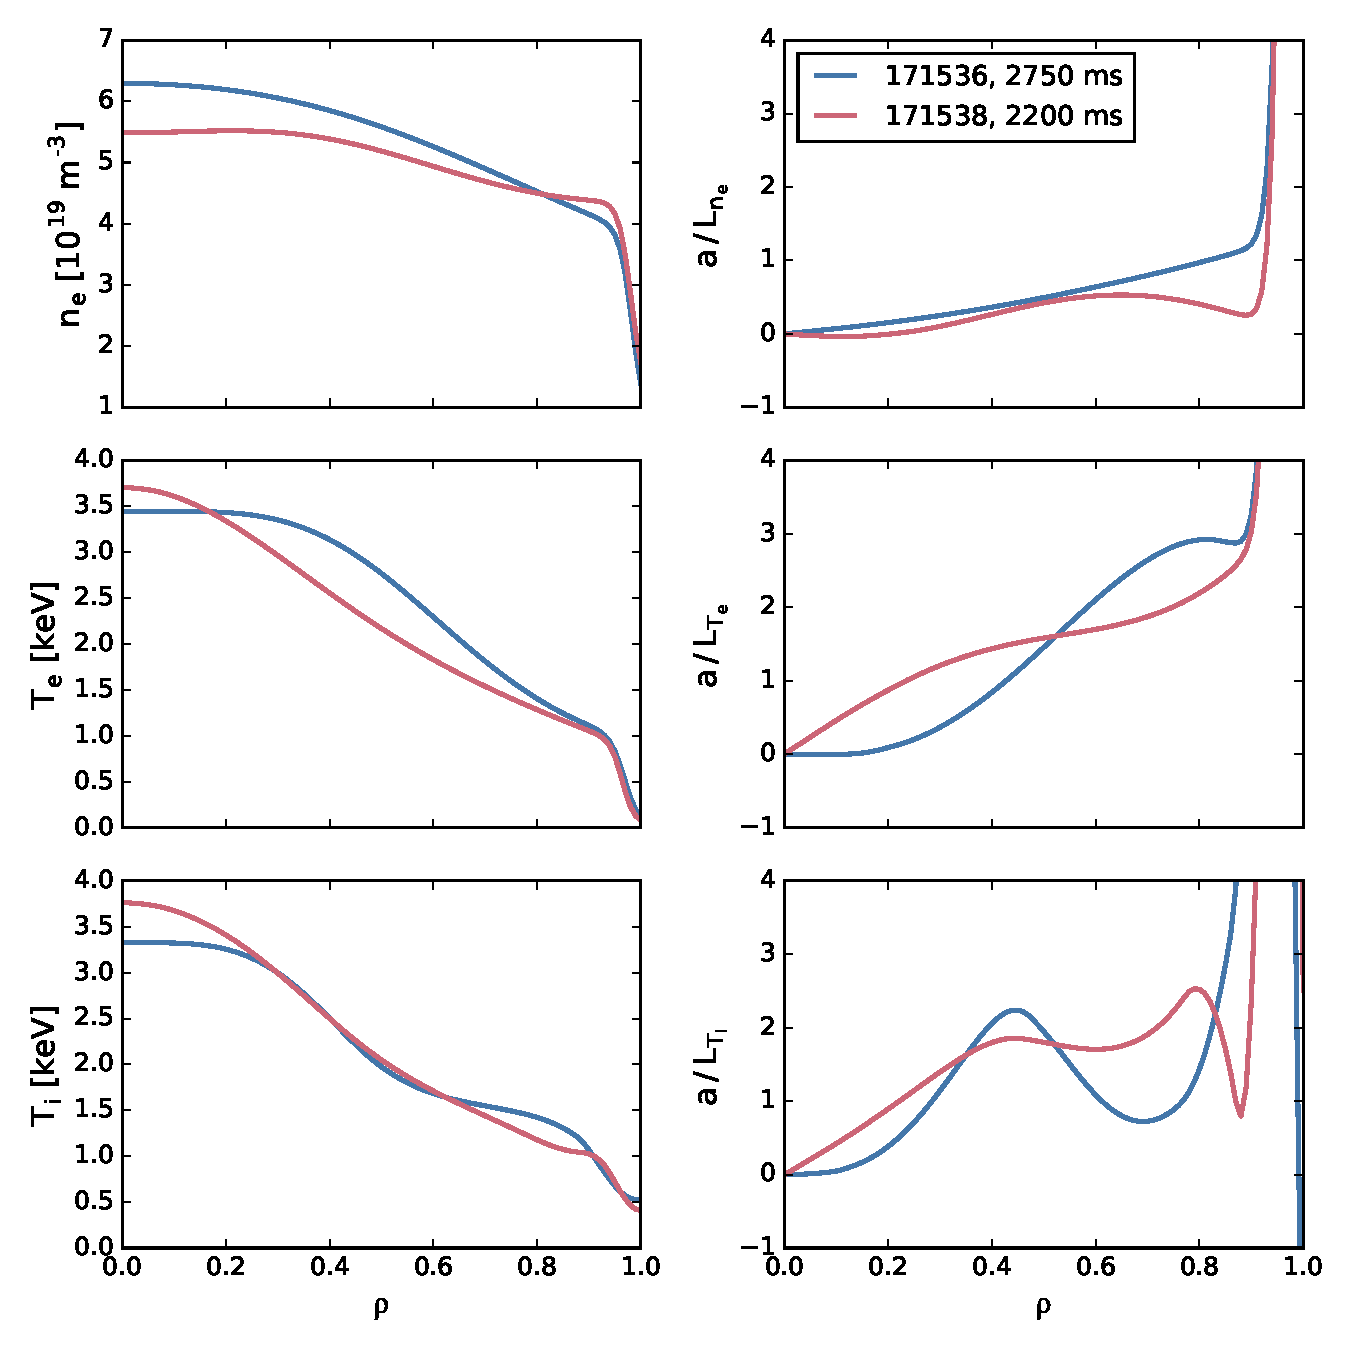
\includegraphics[width = \textwidth]{%
    Chapters/TurbulenceMeasurements/figs/profiles.pdf}
  \caption[Equilibrium profiles, inverse scale lengths, \& $\ExB$ shearing rate]{%
    Profiles, inverse scale lengths, and $\ExB$ shearing rate:
    (a) electron density $n_e$,
    (b) electron temperature $T_e$,
    (c) deuterium temperature $T_i$,
    (d) radial electric field $E_r$ along the outboard midplane,
    (e) normalized inverse $n_e$ scale length $a / L_{n_e}$,
    (f) normalized inverse $T_e$ scale length $a / L_{T_e}$,
    (g) normalized inverse $T_i$ scale length $a / L_{T_i}$,
    (h) $\ExB$ shearing rate $\gamma_E$.
    The shaded bands indicate the $1\sigma$ uncertainties in the profiles,
    as determined by performing separate fits to $100$ distinct data sets
    generated via Monte Carlo variation
    of the measurements about their uncertainties.
    Representative measurements and their uncertainties are indicated
    for a $\SI{10}{\milli\second}$ window from a single shot.
    The relatively large uncertainty on $\gamma_E$
    is dominated by uncertainty in the curvature
    of the $T_i$ profile.
  }
\label{fig:TurbulenceMeasurements:profiles}
\end{figure}

\begin{figure}
  \centering
  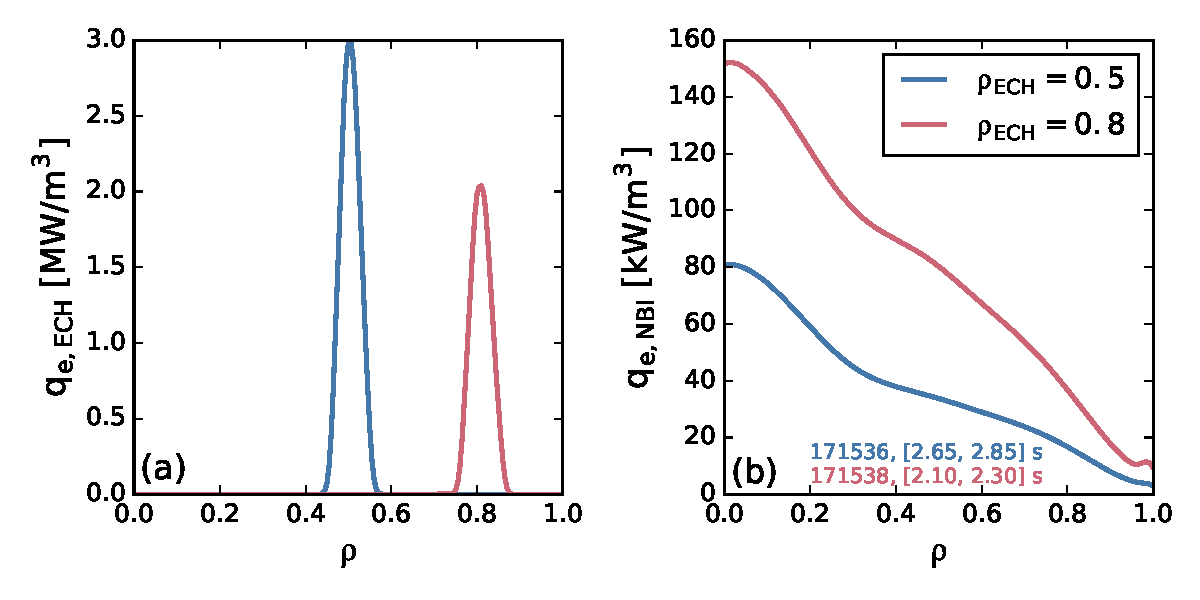
\includegraphics[width = \textwidth]{%
    Chapters/TurbulenceMeasurements/figs/electron_heating.pdf}
  \caption[ECH \& NBI electron-heating profiles]{%
    (a) ECH electron heating density $q_{e,\text{ECH}}$ and
    (b) NBI electron heating density $q_{e,\text{NBI}}$.
    When moving ECH from $\rho = 0.5$ to $\rho = 0.8$,
    maintaining constant $\beta_N$
    requires increased NBI heating
    (see Figure~\ref{fig:TurbulenceMeasurements:traces}(c)),
    which enhances the NBI electron heating density $q_{e,\text{NBI}}$
    across the full plasma profile.
    The radiated power and ohmic heating
    negligibly change between the two discharges.
  }
\label{fig:TurbulenceMeasurements:electron_heating}
\end{figure}


\section{Combined PCI-interferometer measurements}
\label{sec:TurbulenceMeasurements:Measurements}


\subsection{ELM filtering}
\label{sec:TurbulenceMeasurements:ELM_filtering}
Edge localized modes (ELMs) expel impurities from the plasma but
will also present severe challenges to plasma-facing components
in future reactors~\cite[Sec.~7.17]{wesson}.
Because of their virulence and their bursty nature,
ELMs produce strong spiking in the interferometer and PCI measurements,
whitening the measured spectra
[Sec.~10.3.2.3]\cite{bendat_and_piersol}.
Additionally, the temperature and density profiles relax during an ELM,
altering the turbulent drives in the plasma edge.
In order to accurately estimate
the spectrum of the background turbulence, then,
the ELM contributions to the interferometer and PCI measurements
must be removed.

\begin{figure}
  \centering
  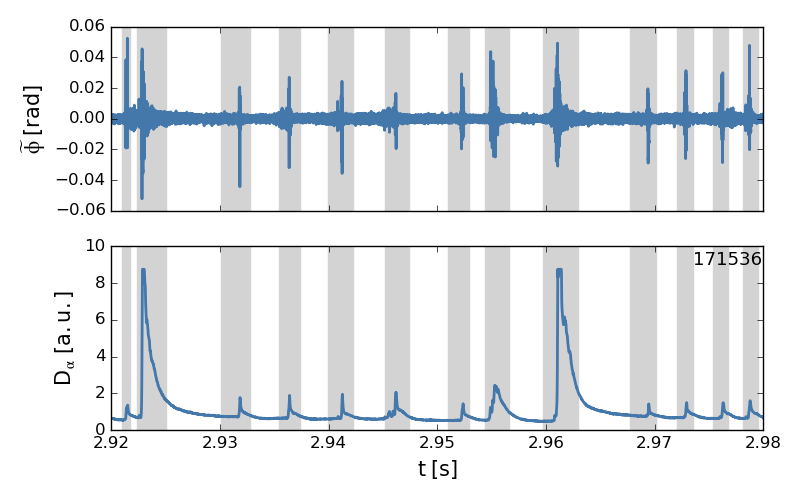
\includegraphics[width = \textwidth]{%
    Chapters/TurbulenceMeasurements/figs/ELM_filtering_example.png}
  \caption[ELM filtering]{%
    Edge localized modes (ELMs) must be removed
    from the PCI and interferometer measurements
    prior to spectral analysis of the background turbulence.
    (Upper panel): The interferometer-measured
    fluctuating phase $\tilde{\phi}$,
    with large, ELM-induced spiking.
    (Lower panel): Divertor $D_{\alpha}$ emission,
    indicating the presence of large Type I ELMs
    as well as smaller ELMs.
    Windows \emph{excluded} from spectral analysis are shown in gray.
    The \diiid\space shot number is shown in the upper right
    of the lower panel.
  }
\label{fig:TurbulenceMeasurements:ELM_filtering_example}
\end{figure}

In this work, ELMs are simply and automatically detected
using measurements from the interferometer.
After the high-pass filtering described in
Section~\ref{sec:Implementation:DataPreparation:high_pass_filtering},
the interferometer-measured fluctuating phase $\tilde{\phi}$
is a zero-mean, random process,
as shown in the upper panel of
Figure~\ref{fig:TurbulenceMeasurements:ELM_filtering_example}.
Large, intermittent spikes pepper $\tilde{\phi}(t)$ during ELMy H-mode, and
the lower panel of
Figure~\ref{fig:TurbulenceMeasurements:ELM_filtering_example}
indicates that these spikes are well correlated
with ELM-induced $D_{\alpha}$ emission in the divertor.
While the $D_{\alpha}$ emission following large Type I ELMs
exhibits a relatively slow decay,
the interferometer-measured $\tilde{\phi}$
returns to stationarity much more rapidly.
Thus, it is desirable to identify
stationary inter-ELM windows
from the interferometer measurements
rather than the $D_{\alpha}$ emission.
Points in the interferometer-measured $\tilde{\phi}$
exceeding $3 \times$ the RMS value
are identified as ELMs, and
successive ELMs are required to be separated
by at least a $\SI{0.5}{\milli\second}$ ``debouncing time''
(spikes separated by less than the debouncing time
are classified as belonging to the same ELM).
Subsequent spectral analysis is then performed
using only the $20\%$ -- $80\%$ inter-ELM windows
of the interferometer and PCI measurements.
Figure~\ref{fig:TurbulenceMeasurements:ELM_filtering_example}
shows the windows \emph{excluded} from spectral analysis in gray.


\subsection{Frequency spectra}
\label{sec:TurbulenceMeasurements:Sf}
One-sided autospectral densities estimates $G_{\phi,\phi}(f)$
of the phase fluctuations
are calculated using the methodology
described in Section~\ref{app:SpectralEstimation:NonParametric}.
The interferometer and PCI signals
from the shaded windows in
Figure~\ref{fig:TurbulenceMeasurements:traces}
are split into realizations of $1024$ points
(corresponding to roughly $\SI{250}{\micro\second}$)
resulting in a frequency resolution
of approximately $\SI{4}{\kilo\hertz}$ in the spectral estimates.
As described in Section~\ref{sec:TurbulenceMeasurements:ELM_filtering},
only realizations falling within
$20\%$ -- $80\%$ of each inter-ELM window
are included in the ensemble averaging;
the exact number of realizations $N_r$
included in each ensemble
depends on the details of the ELM dynamics, but
$N_r \sim 900$ for the shots considered here,
corresponding to a relative random error
in $G_{\phi,\phi}(f)$ of approximately $3\%$.
A Hanning window is applied to each realization
prior to computation of its fast Fourier transform (FFT).
To simplify inter-ELM bookkeeping,
adjacent realizations have zero overlap.
As described in
Section~\ref{sec:Implementation:DataPreparation:high_pass_filtering},
the interferometer and PCI phase signals
are high-pass filtered prior to spectral analysis, and
no further detrending is performed.
The resulting spectral estimates
for $\rho_{\text{ECH}} = 0.5$ and $\rho_{\text{ECH}} = 0.8$
are shown in
Figure~\ref{fig:TurbulenceMeasurements:Sf_interferometer_pci}.
The corresponding noise floors are estimated
from $\SI{50}{\milli\second}$ of data
prior to plasma breakdown;
the knee in the PCI noise floor
at approximately $\SI{500}{\kilo\hertz}$
corresponds to the roll-off in the temporal bandwidth
of the PCI detector and its preamplifiers.
As expected theoretically
(see Figure~\ref{fig:InterferometricMethods:interferometric_method_transfer_functions})
and observed empirically in sound-wave calibrations
(see Figure~\ref{fig:Implementation:cross_calibration}),
the PCI is more sensitive than the heterodyne interferometer.

\begin{figure}
  \centering
  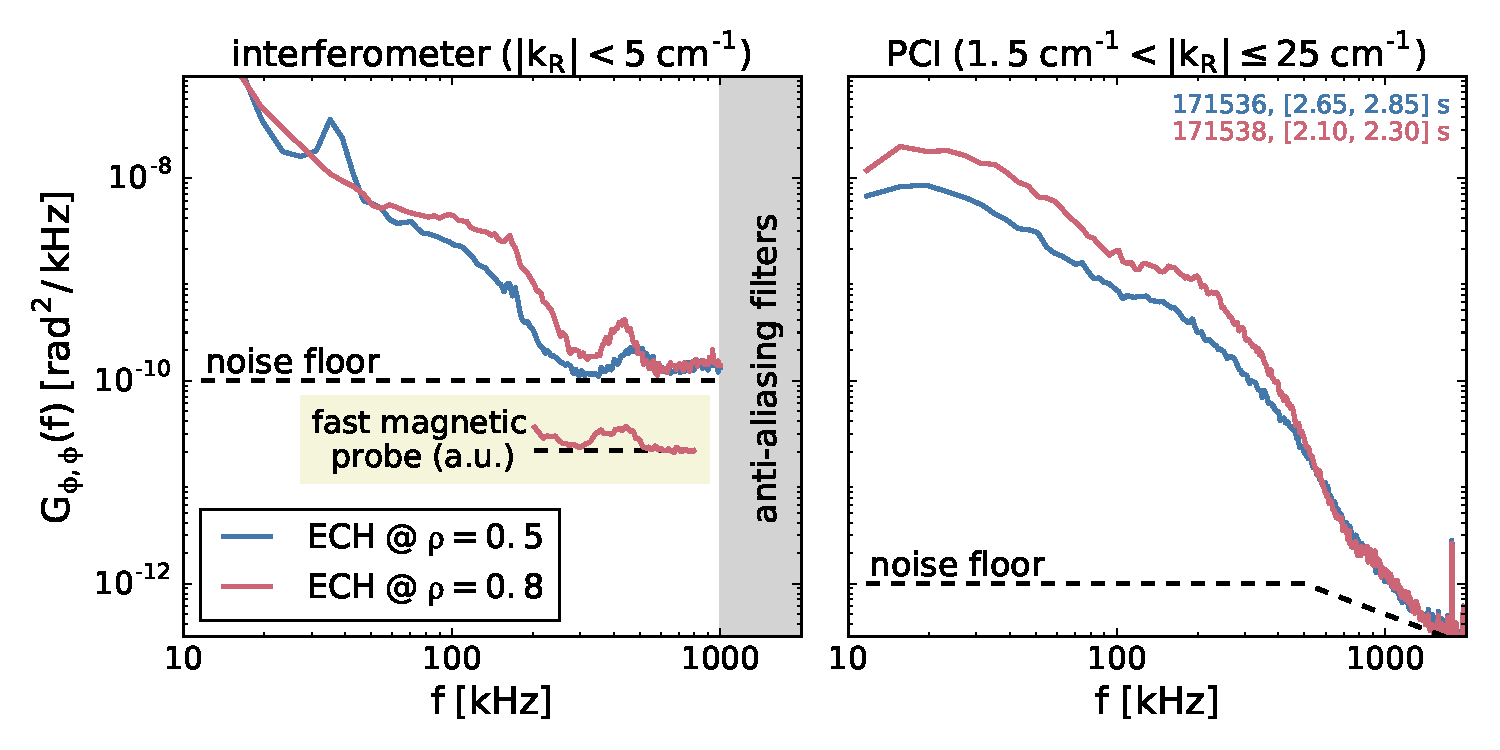
\includegraphics[width = \textwidth]{%
    Chapters/TurbulenceMeasurements/figs/Sf_interferometer_pci.pdf}
  \caption[Interferometer \& PCI frequency spectra]{%
    Interferometer and PCI frequency spectra.
  }
\label{fig:TurbulenceMeasurements:Sf_interferometer_pci}
\end{figure}

Interestingly, the autospectral density of the heterodyne interferometer
indicates the presence of a distinct broadband fluctuation
with a central frequency $f_0 \sim \SI{450}{\kilo\hertz}$ and
a bandwidth $\Delta f \sim \SI{300}{\kilo\hertz}$.
This fluctuation is larger than
the corresponding PCI-measured fluctuations
in this frequency range, but
it is absent from the autospectral density of the PCI;
this indicates that the fluctuation wavenumber
is smaller than the PCI low-$k$ cutoff
(\ref{eq:Implementation:kg_realized}).
\begin{itemize}
  \item Magnetic component, as shown in inset
  \item Total power $\text{var}(\tilde{\phi})$ in fluctuation
    robustly increases when moving $\rho_{\text{ECH}} = 0.5$ to
    $\rho_{\text{ECH}} = 0.8$, as shown in
    Figure~\ref{fig:TurbulenceMeasurements:interferometer_bump_integrated_power}
  \item The collisionality increases (\textcolor{red}{how much?})
    over the PCI measurable domain, as shown in
    Figure~\ref{fig:TurbulenceMeasurements:collisionality}
  \item Microtearing mode predicted to be marginally unstable
    in reference discharge~\cite{holland_nf17}
\end{itemize}

\begin{figure}
  \centering
  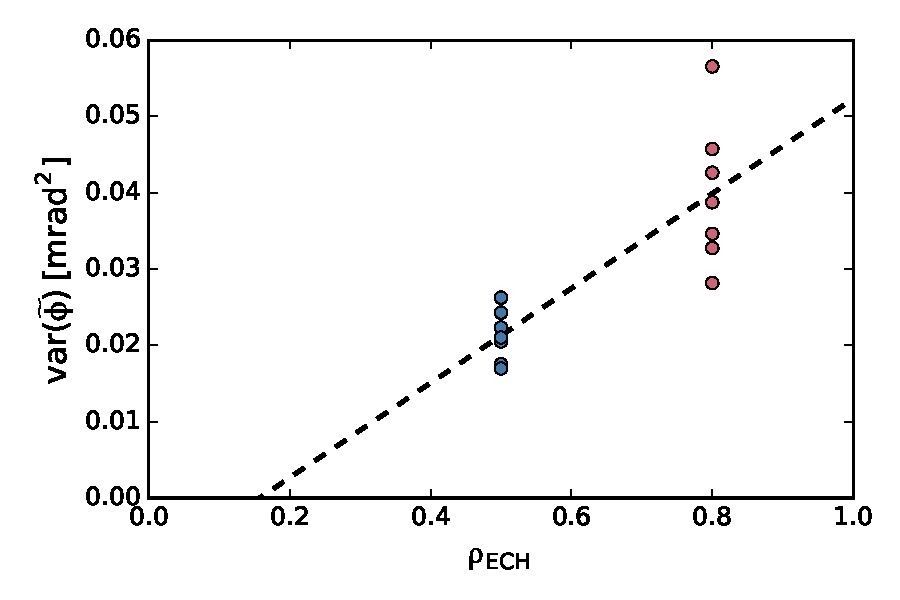
\includegraphics[width = 0.75 \textwidth]{%
    Chapters/TurbulenceMeasurements/figs/interferometer_bump_integrated_power.pdf}
  \caption[Power in low-$k$, mid-$f$ turbulence vs. ECH location]{%
    Power $\text{var}(\tilde{\phi})$ in interferometer-measured
    low-$k$, mid-$f$ turbulence vs. ECH location $\rho_{\text{ECH}}$.
    Powers are estimated by integrating the interferometer's
    one-sided autospectral densities
    (e.g.\ those shown in the left panel of
    Figure~\ref{fig:TurbulenceMeasurements:Sf_interferometer_pci})
    between $\SI{300}{\kilo\hertz}$ and $\SI{600}{\kilo\hertz}$.
    Different points correspond to different shots
    from the multiscale experiment, and
    the dashed line is the linear least-squares fit to the points.
  }
\label{fig:TurbulenceMeasurements:interferometer_bump_integrated_power}
\end{figure}

\begin{figure}
  \centering
  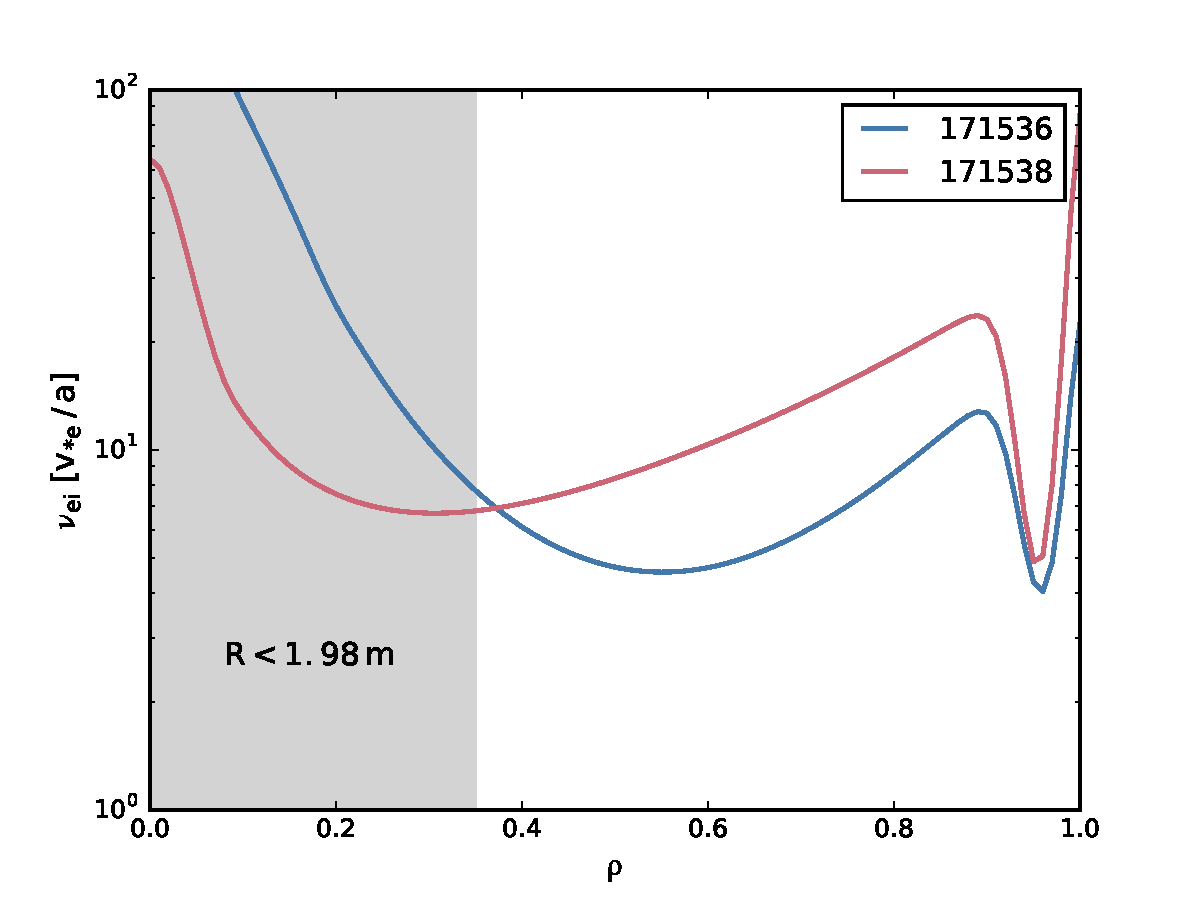
\includegraphics[width = 0.9 \textwidth]{%
    Chapters/TurbulenceMeasurements/figs/collisionality.pdf}
  \caption[Collisionality variation with ECH location]{%
    Collisionality variation with ECH location.
  }
\label{fig:TurbulenceMeasurements:collisionality}
\end{figure}

The interferometer- and PCI-measured frequency spectra
reveal a rich set of plasma dynamics.
Both systems measure a distinct increase \textcolor{red}{(how much?)}
in low-frequency ($f \lesssim \SI{300}{\kilo\hertz}$) broadband fluctuations
when moving ECH from $\rho = 0.5$ to $\rho = 0.8$,
which may be responsible for the slightly reduced confinement
in Figure~\ref{fig:TurbulenceMeasurements:traces}(g).
The \textcolor{red}{magnitude-squared coherence $\gamma^2_{xy}$}
between the interferometer and PCI measurements
is shown in Figure~\ref{fig:TurbulenceMeasurements:gamma2xy}.
The magnitude-squared coherence quantifies
the overlap between the interferometer and PCI signals,
with $\gamma^2_{xy} = 0$ indicating $0\%$ overlap and
$\gamma^2_{xy} = 1$ indicating $100\%$ overlap.
Interestingly, for $f \lesssim \SI{100}{\kilo\hertz}$,
the coherence is low,
indicating that the majority of this signal
consists of low-$k$ fluctuations invisible to the PCI.
Between $\SI{100}{\kilo\hertz} \lesssim f \lesssim \SI{300}{\kilo\hertz}$
approximately \textcolor{red}{$65\%$}
of the fluctuations sit in the mid-$k$ overlap
of the interferometer and the PCI.
\graffito{\textcolor{red}{better explanation}}
Moving ECH from $\rho = 0.5$ to $\rho = 0.8$
increases the coherence for $f \gtrsim \SI{200}{\kilo\hertz}$,
suggesting that the wavenumbers are reduced.
For $f \gtrsim \SI{300}{\kilo\hertz}$,
there is no common signal between the interferometer and PCI.
The PCI measures a small but physical fluctuation increase
at $f \sim \SI{1}{\mega\hertz}$
when ECH moves from $\rho = 0.5$ to $\rho = 0.8$;
Section~\ref{sec:TurbulenceMeasurements:Skf}
shows that this corresponds to a distinct turbulent branch.
This turbulent branch sits
below the noise floor of the interferometer and
at the temporal-bandwidth limits of the interferometer's
current anti-aliasing filters.

\begin{figure}
  \centering
  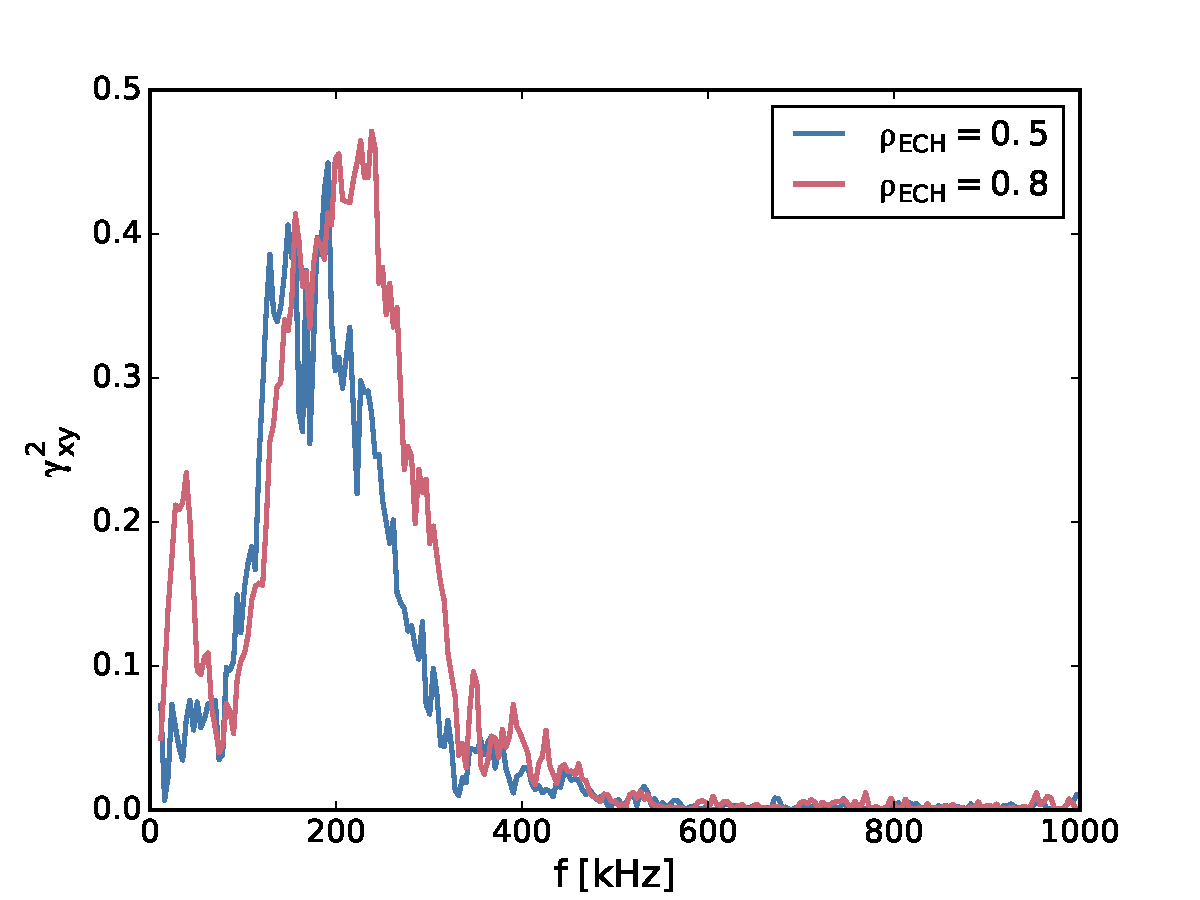
\includegraphics[width = \textwidth]{%
    Chapters/TurbulenceMeasurements/figs/coherence.pdf}
  \caption[Magnitude-squared coherence]{%
    Magnitude-squared coherence $\gamma^2_{xy}$
    between interferometer and PCI measurements.
  }
  \label{fig:TurbulenceMeasurements:gamma2xy}
\end{figure}


\subsection{Frequency-wavenumber spectra}
\label{sec:TurbulenceMeasurements:Skf}

\begin{figure}
  \centering
  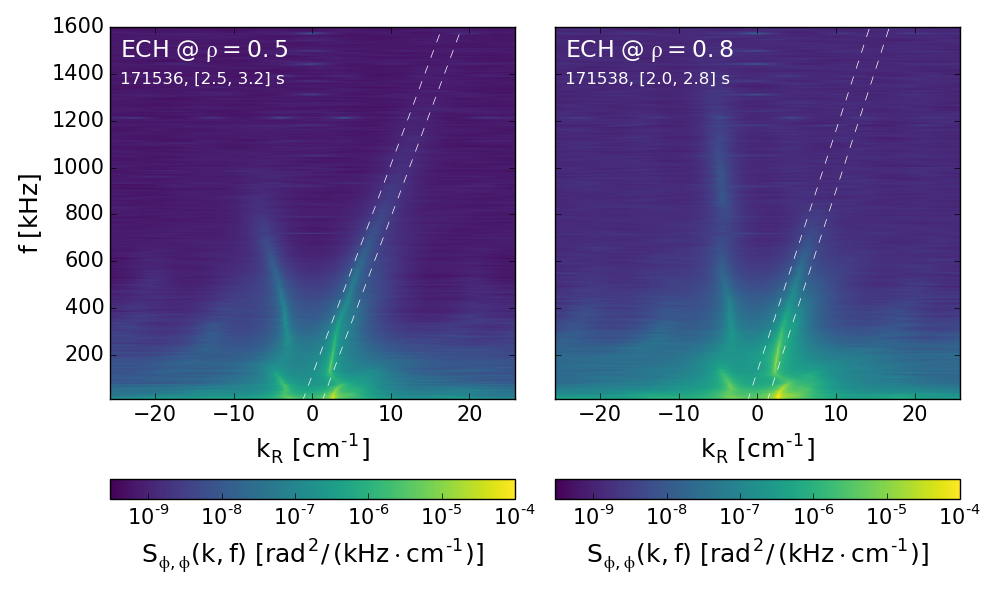
\includegraphics[width = \textwidth]{%
    Chapters/TurbulenceMeasurements/figs/Skf_pci.png}
  \caption[PCI frequency-wavenumber spectra]{%
    PCI frequency-wavenumber spectra. $p = 6$.
  }
\label{fig:TurbulenceMeasurements:Skf_pci}
\end{figure}


\subsection{Wavenumber spectra}
\label{sec:TurbulenceMeasurements:Sk}
\begin{figure}
  \centering
  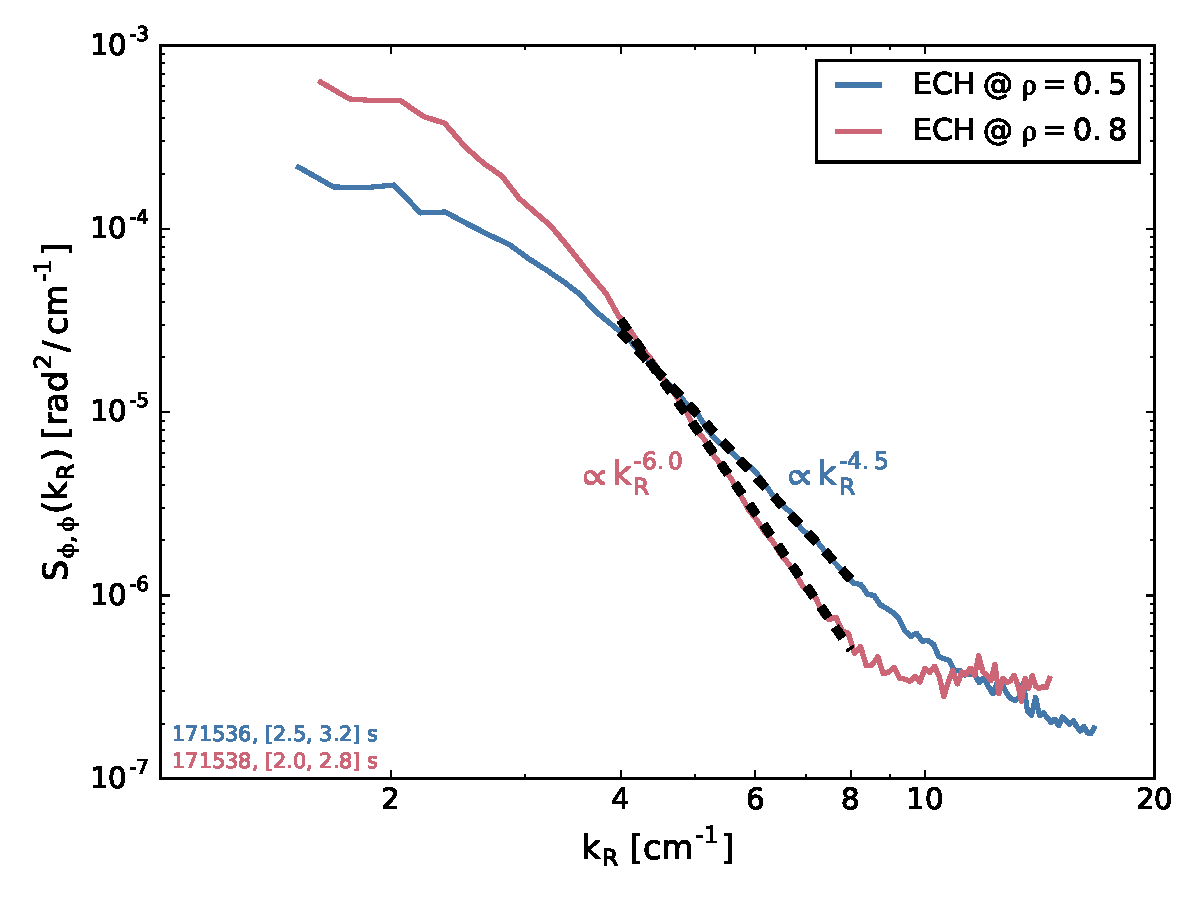
\includegraphics[width = 0.9 \textwidth]{%
    Chapters/TurbulenceMeasurements/figs/Sk_power_law.pdf}
  \caption[PCI-measured power law]{%
    PCI-measured power law from branches annotated in
    Figure~\ref{fig:TurbulenceMeasurements:Skf_pci}.
  }
\label{fig:TurbulenceMeasurements:Sk_power_law}
\end{figure}


\subsection{Doppler-shift localization of high-$k$ turbulence}
As a line-integrated measurement,
PCI is sensitive to fluctuations with wavevectors $\vect{k}$
that are perpendicular to the beam path
(i.e.\ $\vect{k} \perp \zhat$
for the vertical beam path of \diiid's PCI).
Further, fluctuations are strongly field-aligned
such that they are approximately perpendicular
to the local magnetic field;
assuming the fluctuations are electrostatic,
the local magnetic field is well-represented
by the equilibrium field $\Beq$ such that
$\vect{k} \perp \Beq$.
Thus, the wavevector satisfies
\begin{equation}
  \vect{k}
  \propto
  \zhat \cross \beq,
  \label{eq:TurbulenceMeasurements:kpropto}
\end{equation}
where $\beq = \Beq / |\Beq|$ is the unit vector
in the direction of the local equilibrium magnetic field.
Thus, the PCI-measured fluctuations have wavevectors
\begin{equation}
  \vect{k}
  =
  (\vect{k} \cdot \khat) \khat,
\end{equation}
where
\begin{equation}
  \khat
  =
  \frac{\zhat \cross \beq}{|\zhat \cross \beq|}
  \label{eq:TurbulenceMeasurements:khat}.
\end{equation}
For a tokamak with a dominant toroidal magnetic field,
$\beq \sim \zetahat$ and
$|\zhat \cross \beq| \sim 1$ such that
(\ref{eq:TurbulenceMeasurements:khat}) is never singular.
Noting the $(R, z, \zeta)$ and $(\rho, \theta, \zeta)$
coordinate systems defined in
Fig.~\ref{fig:TurbulenceMeasurements:coordinate_geometry} and
explicitly writing the equilibrium magnetic field
as the sum of its toroidal and poloidal components
$\Beq = B_{\zeta} \zetahat + B_{\theta} \thetahat$,
the unit vector (\ref{eq:TurbulenceMeasurements:khat})
can be explicitly written as
\begin{equation}
  \khat
  =
  \frac{%
    B_{\zeta} \Rhat + (B_{\theta} \sin\theta) \zetahat}{%
    {\left[ B_{\zeta}^2 + {(B_{\theta} \sin\theta)}^2 \right]}^{1/2}}.
  \label{eq:TurbulenceMeasurements:khat_explicit}
\end{equation}
Because $|B_{\theta}| \ll |B_{\zeta}|$,
the wavevectors are predominantly in the major-radial direction,
i.e.\ $\khat \sim \Rhat$.

\begin{figure}
  \centering
  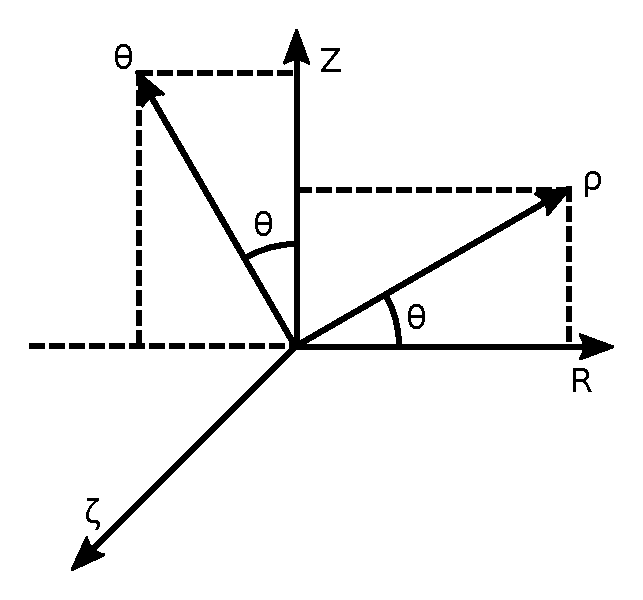
\includegraphics[width = 0.5 \textwidth]{%
    Chapters/TurbulenceMeasurements/figs/coordinate_geometry.pdf}
  \caption[Measurement coordinate system]{%
    Measurement coordinate system.
    Here, $R$ is the major-radial direction,
    $z$ is the lab-frame vertical direction,
    $\zeta$ is the toroidal angle,
    $\theta$ is the poloidal angle, and
    $\rho$ is a flux-surface label
    corresponding to the square root
    of the normalized toroidal magnetic-field flux.
  }
\label{fig:TurbulenceMeasurements:coordinate_geometry}
\end{figure}

Now, assuming that $\ExB$ advection
is the predominant contribution
to the PCI-measured phase velocity,
the line-integrated PCI measurements can be moderately localized.
To see this, note that the PCI measurements are Doppler shifted by
$\Delta \omega = \vect{k} \cdot \vect{v}$,
where $\vect{v}$ is the lab-frame velocity of the plasma.
Because $\vect{k} \perp \Beq$ by
(\ref{eq:TurbulenceMeasurements:kpropto}),
$\vect{k} \cdot \vect{v} = \vect{k} \cdot \vperp$, where
$\vperp$ is the velocity
perpendicular to the equilibrium magnetic field.
Defining the plasma frame via the ideal-MHD relation
$\vect{E} + \vperp \cross \Beq = 0$,
the perpendicular velocity is simply the $\ExB$ velocity
i.e.\ $\vperp = \vExB$.
Now, the electrostatic potential $\varphi = \varphi(\rho)$
is a flux function such that
the corresponding electric field is
$\vect{E} = -\nabla \varphi = E_r(\rho, \theta) \rhohat$.
The resulting $\ExB$ velocity is
\begin{align}
  \vExB
  =
  \frac{\vect{E} \times \Beq}{B_0^2}
  % \notag \\
  =
  \frac{E_r(\rho, \theta)}{B_0^2}
  \left(%
    B_{\theta} \zetahat
    -
    B_{\zeta} \thetahat
  \right)
  \label{eq:TurbulenceMeasurements:vExB}
\end{align}
such that the Doppler shift
$\Delta \omega = \vect{k} \cdot \vExB$ becomes
\begin{equation}
  \Delta \omega
  =
  \frac{%
    (\vect{k} \cdot \khat) E_r(\rho, \theta) \sin\theta}{%
    {\left[ B_{\zeta}^2 + {(B_{\theta} \sin\theta)}^2 \right]}^{1/2}}.
  \label{eq:TurbulenceMeasurements:Doppler_shift_from_ExB}
\end{equation}
Thus, the plasma's $\ExB$ rotation
results in a PCI-measured phase velocity
\begin{align}
  \vpciE
  =
  \frac{\Delta \omega}{k}
  =
  \frac{%
    \sgn(\vect{k} \cdot \khat) E_r(\rho, \theta) \sin\theta}{%
    {\left[ B_{\zeta}^2 + {(B_{\theta} \sin\theta)}^2 \right]}^{1/2}},
  \label{eq:TurbulenceMeasurements:PCI_phase_velocity_from_ExB}
\end{align}
where the sign function $\sgn(x)$
returns the sign of argument $x$.
Here, the plasma-frame phase velocity $v_{\text{ph}}$
of the fluctuations have been neglected,
which is valid when $|v_{\text{ph}}| \ll |\vpciE|$.
Further, note that the polarity of $\sin\theta$
switches at the plasma midplane (where $\theta = 0$) such that
(\ref{eq:TurbulenceMeasurements:PCI_phase_velocity_from_ExB})
switches signs when passing from above the plasma midplane
to below the plasma midplane.
Figure~\ref{fig:TurbulenceMeasurements:doppler_shift}
compares $\vpciE$ from
(\ref{eq:TurbulenceMeasurements:PCI_phase_velocity_from_ExB})
to the measured phase velocity $\vpcimeas$
of the high-$k$ turbulence observed in the left panel of
Figure~\ref{fig:TurbulenceMeasurements:Skf_pci}.

\begin{figure}
  \centering
  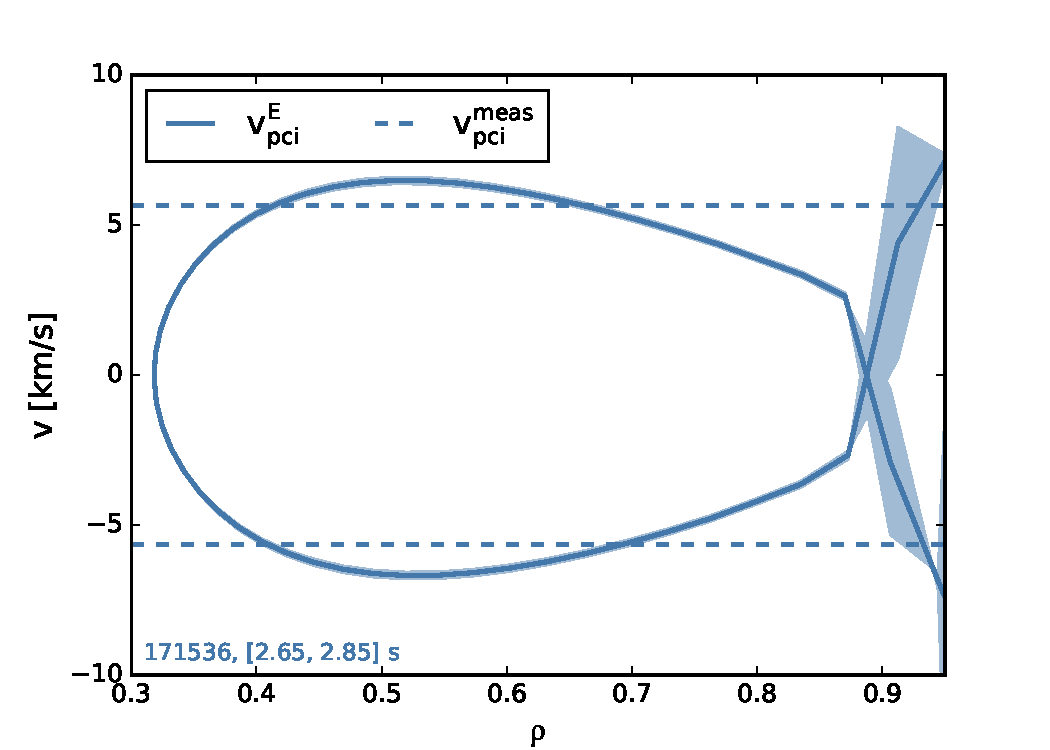
\includegraphics[width = 0.9 \textwidth]{%
    Chapters/TurbulenceMeasurements/figs/doppler_shift.pdf}
  \caption[Doppler-shift localization of high-$k$ turbulence]{%
    A comparison of the $\ExB$-induced phase velocity $\vpciE$ from
    (\ref{eq:TurbulenceMeasurements:PCI_phase_velocity_from_ExB})
    to the measured phase velocity $\vpcimeas$
    of the high-$k$ turbulence observed in the left panel
    of Figure~\ref{fig:TurbulenceMeasurements:Skf_pci}.
    The near degeneracy of $\vpciE$ with $\rho$
    corresponds to propagation above and below the plasma midplane.
    As the spatially filtering ``mask''~\cite{dorris_phd, dorris_rsi09}
    was not used in this experiment,
    it is not possible to determine whether
    $\vpcimeas$ corresponds to propagation above or below the midplane, so
    both $\vpcimeas$ and $-\vpcimeas$ are plotted.
  }
\label{fig:TurbulenceMeasurements:doppler_shift}
\end{figure}

As a brief aside, it should be emphasized
that the radial electric field $E_r$
in (\ref{eq:TurbulenceMeasurements:PCI_phase_velocity_from_ExB})
is \emph{not} a flux function.
To see this, recall that
the corresponding electrostatic potential
\emph{is} a flux function,
i.e.\ $\varphi = \varphi(\rho) = \varphi(\psi)$,
where $\psi$ is the flux-surface label
corresponding to the poloidal magnetic-field flux per radian.
Now,
\begin{align}
  E_r(\rho, \theta)
  &=
  -\left( \frac{\partial\varphi}{\partial r} \right)
  \notag \\
  &=
  -\left( \frac{d\varphi}{d\psi} \right)
  \left( \frac{\partial\psi}{\partial r} \right)
  \notag \\
  &=
  -\left( \frac{d\varphi}{d\psi} \right)
  \left( R B_{\theta} \right),
\end{align}
where the last line follows from the definition
of $\psi$ as the poloidal magnetic-field flux per radian.
The derivative $d\varphi / d\psi$
is a flux function because $\varphi$ is a flux function, and
this implies that $E_r / (R B_{\theta})$ is also a flux function.
Thus, the radial electric field at any point
within the last closed flux surface can be computed
from the radial electric field
along the outboard midplane (where $\theta = 0$) as follows
\begin{equation}
  \left.
  \frac{E_r}{R B_{\theta}}
  \right|_{\rho, \theta}
  =
  \left.
  \frac{E_r}{R B_{\theta}}
  \right|_{\rho, \theta = 0}.
  \label{eq:TurbulenceMeasurements:radial_electric_field}
\end{equation}


\section{TGLF modeling}
\begin{figure}[h!]
  \centering
  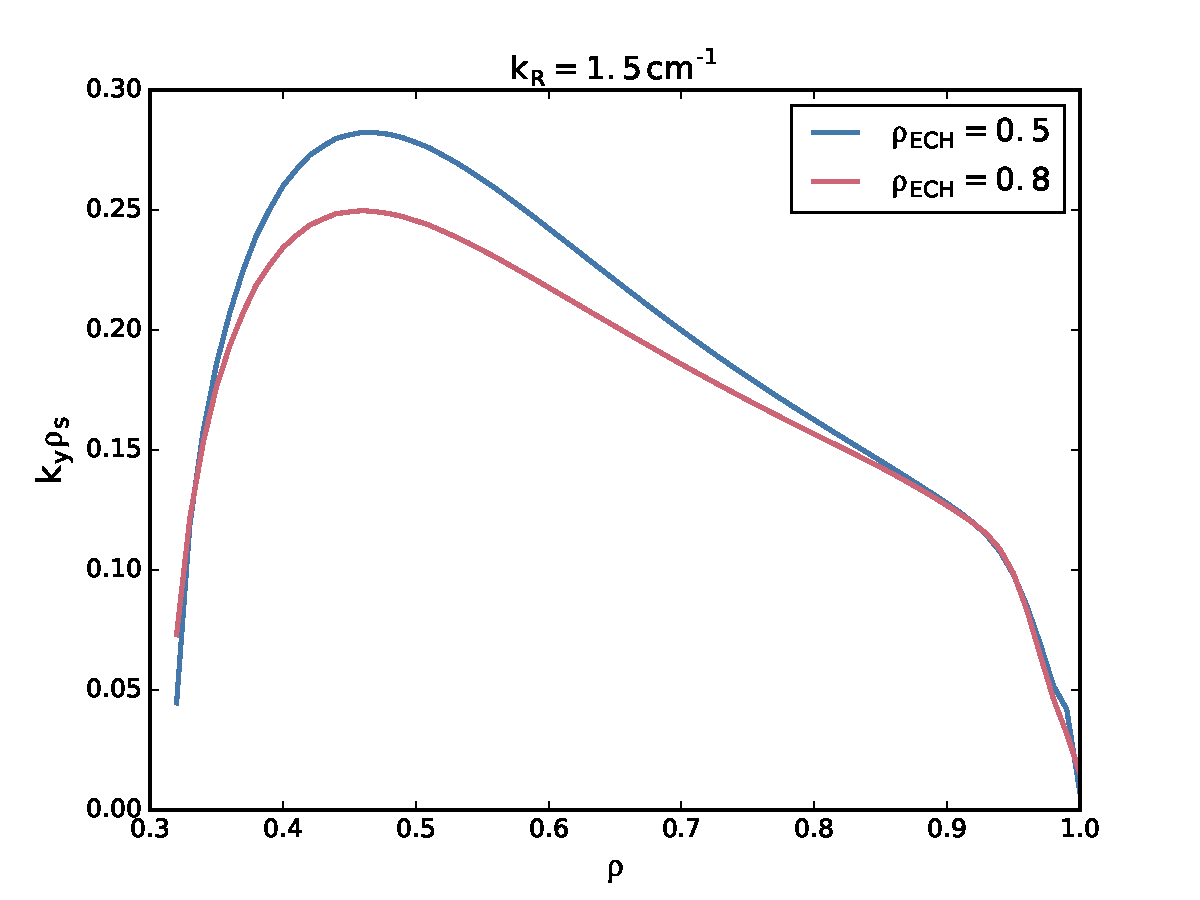
\includegraphics[width = \textwidth]{%
    Chapters/TurbulenceMeasurements/figs/wavenumber_conversion.pdf}
  \caption[Profiles of $k_y \rho_s$ for $k_R = \SI{1.5}{\per\centi\meter}$]{%
    Profiles of $k_y \rho_s$ for $k_R = \SI{1.5}{\per\centi\meter}$.
  }
\label{fig:TurbulenceMeasurements:wavenumber_conversion}
\end{figure}

\begin{figure}[h!]
  \centering
  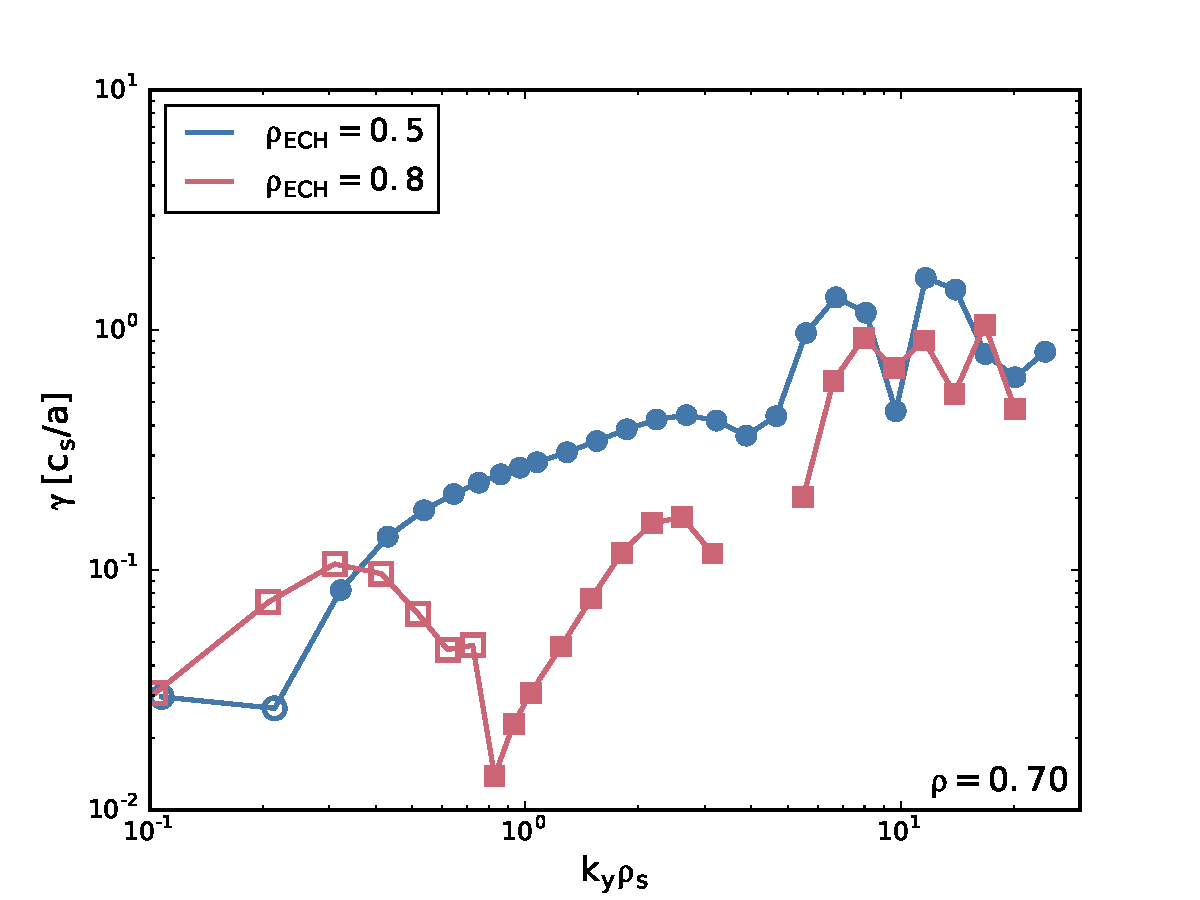
\includegraphics[width = \textwidth]{%
    Chapters/TurbulenceMeasurements/figs/linear_stability_rho070.pdf}
  \caption[TGLF-predicted linear growth rates]{%
    TGLF-predicted linear growth rates.
    Filled symbols indicate electron modes, while
    unfilled symbols indicate ion modes.
  }
\label{fig:TurbulenceMeasurements:linear_stability}
\end{figure}

\begin{figure}[h!]
  \centering
  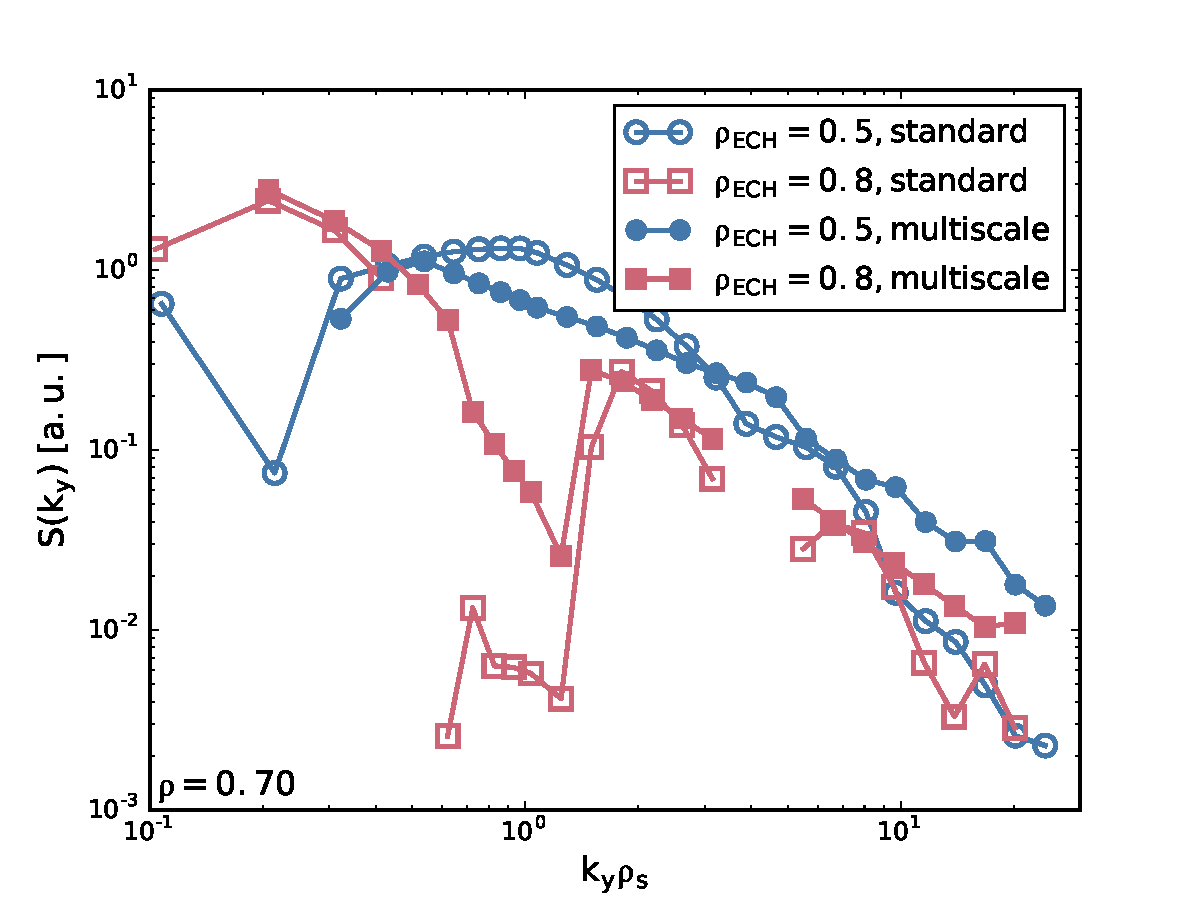
\includegraphics[width = \textwidth]{%
    Chapters/TurbulenceMeasurements/figs/density_spectra_rho070.pdf}
  \caption[TGLF-predicted density-fluctuation spectra]{%
    TGLF-predicted density-fluctuation spectra
  }
\label{fig:TurbulenceMeasurements:density_spectra}
\end{figure}


\bibliographystyle{plainurl}
\bibliography{references}
